%!TEX platex=1
\documentclass[11pt,xcolor=dvipsnames,table,dvipdfmx]{beamer}
\usepackage{amsmath, amssymb}
\usepackage{latexsym}
\usepackage{ascmac}
\usepackage{bm}

%Beamer$B$N@_Dj(B
\usetheme{Boadilla}
%Beamer$B%U%)%s%H@_Dj(B
\usepackage{txfonts} % TX$B%U%)%s%H(B
\usepackage[deluxe]{otf} % $BF|K\8lB?%&%'%$%H2=(B
\renewcommand{\familydefault}{\sfdefault}  % $B1QJ8$r%5%s%;%j%UBN$K(B
\renewcommand{\kanjifamilydefault}{\gtdefault}  % $BF|K\8l$r%4%7%C%/BN$K(B
\usefonttheme{professionalfonts}
\setbeamerfont{alerted text}{series=\bfseries} % Alert$B$rB@;z(B
\setbeamerfont{section in toc}{series=\mdseries} % $BL\<!$OB@;z$K$7$J$$(B
\setbeamerfont{frametitle}{size=\Large} % $B%U%l!<%`%?%$%H%kJ8;z%5%$%:(B
\setbeamerfont{title}{size=\LARGE} % $B%?%$%H%kJ8;z%5%$%:(B
\setbeamerfont{date}{size=\small}  % $BF|IUJ8;z%5%$%:(B

%Beamer$B?'@_Dj(B
\definecolor{UniBlue}{RGB}{0,150,200} 
\definecolor{AlertOrange}{RGB}{255,76,0}
\definecolor{AlmostBlack}{RGB}{38,38,38}
\setbeamercolor{normal text}{fg=AlmostBlack}  % $BK\J8%+%i!<(B
\setbeamercolor{structure}{fg=UniBlue} % $B8+=P$7%+%i!<(B
\setbeamercolor{block title}{fg=UniBlue!50!black} % $B%V%m%C%/ItJ,%?%$%H%k%+%i!<(B
\setbeamercolor{alerted text}{fg=AlertOrange} % \alert $BJ8;z%+%i!<(B
\mode<beamer>{
    \definecolor{BackGroundGray}{RGB}{254,254,254}
    \setbeamercolor{background canvas}{bg=BackGroundGray} % $B%9%i%$%I%b!<%I$N$_GX7J$r$o$:$+$K%0%l!<$K$9$k(B
}

%$B%U%i%C%H%G%6%$%s2=(B
\setbeamertemplate{blocks}[rounded] % Block$B$N1F$r>C$9(B
\useinnertheme{circles} % $B2U>r=q$-$r%7%s%W%k$K(B
\setbeamertemplate{navigation symbols}{} % $B%J%S%2!<%7%g%s%7%s%\%k$r>C$9(B
\setbeamertemplate{footline}[frame number] % $B%U%C%?!<$O%9%i%$%IHV9f$N$_(B

%$B%?%$%H%k%Z!<%8(B
\setbeamertemplate{title page}{%
    \vspace{2.5em}
    {\usebeamerfont{title} \usebeamercolor[fg]{title} \inserttitle \par}
    {\usebeamerfont{subtitle}\usebeamercolor[fg]{subtitle}\insertsubtitle \par}
    \vspace{1.5em}
    \begin{flushright}
        \usebeamerfont{author}\insertauthor\par
        \usebeamerfont{institute}\insertinstitute \par
        \vspace{3em}
        \usebeamerfont{date}\insertdate\par
        \usebeamercolor[fg]{titlegraphic}\inserttitlegraphic
    \end{flushright}
}

% graphicx.sty
\usepackage{graphicx}

%
\def\qed{\hfill $\Box$}

\AtBeginSection[]{
    \frame{\tableofcontents[currentsection, hideallsubsections]} %$BL\<!%9%i%$%I(B
}

%$B%?%$%H%k(B
\title{Monthly Meeting on October}
\author{\textbf{Yuichiro Honda}}
\date{2016/10/05}
\institute{Morita lab. M1}

\begin{document}
\maketitle

\section{Previous work}
\begin{frame}{Last month}
 \begin{enumerate}
  \item searched an (polynomial) algorithm to partition two matroids into their common bases
  \item found an algorithm to find all common bases in two matroids in $O(n(n^2+t)\lambda)$
 \end{enumerate}
\end{frame}



\section{Progress}
\begin{frame}{References}
 \begin{thebibliography}{9}
  \bibitem{1}
	\small{Komei Fukuda, Makoto Namiki: ``Finding all common bases in two matroids'', Discrete Applied Mathmatics 56 (1995) 231-243}
 \end{thebibliography}
\end{frame}

\begin{frame}{Finding all common bases in two matroids}
 \begin{block}{Main result}
  Given two matroids $M_1 = (E, \mathcal{B}_1)$, $M_2 = (E, \mathcal{B}_2)$, and a common base $B^1 \in \mathcal{B}_1 \cap \mathcal{B}_2$, there is an algorithm finding all common bases of them in \alert{$O(n(n^2+t)\lambda)$ }where $\lambda$ is number of the bases and $t$ is the time to make one pivot operation.
 \end{block}
\end{frame}

\begin{frame}{Finding all common bases in two matroids}
 \begin{itemize}
  \item The algorithm use enumeration tree whose height is $|E| = n$ and the height is indexed in descending order from the root
  \item In the beginning, the initial comon base $B^1$ is placed at right most position
  \item $n$-dimentional vector \alert{$P$} $\in \{L,\,R\}^n$ is used to indicate the current position
  \item also current branch is indicated by \alert{$f$} $\in E$
  \item Each one step of algorithm, \alert{$B^k$} goes left updating $B^k$ to $B^{k+1}$ if exists
 \end{itemize}
\end{frame}

\begin{frame}{Finding all common bases in two matroids}
 example:
 \begin{figure}
  \centering
  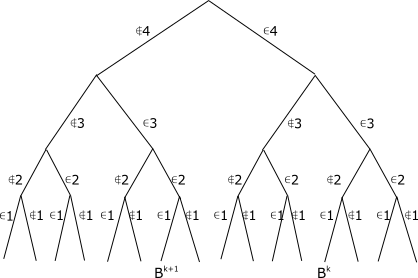
\includegraphics[width=7cm]{text4989-10.png}\vspace{0.3cm}\\
  when the current base $B^k = \{1,\,3,\,4\}$ is placed like above,\\$P = (L\,L\,R\,R)$ and $f = 3$ 
 \end{figure}
\end{frame}

\begin{frame}{Finding all common bases in two matroids}
 next, we need a theorem to reduce the search space like a backtracking
 \begin{figure}
  \centering
  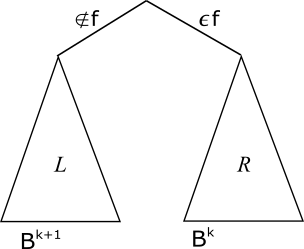
\includegraphics[width=5.2cm]{text4989-7.png}
 \end{figure}
\end{frame}

\begin{frame}{Finding all common bases in two matroids}
 \begin{figure}
  bipartite graph $G(B^k)$\vspace{1cm}\\
  \centering
  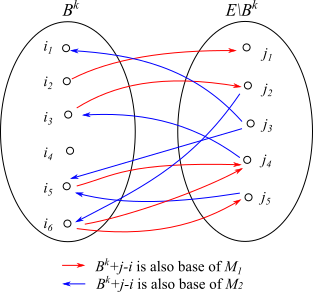
\includegraphics[width=6cm]{text8631-16-2-7.png}
 \end{figure}
\end{frame}

\begin{frame}{Finding all common bases in two matroids}
 \begin{block}{Theorem 1}
  There exists a common base $B^{k+1}$ in $L$ if and only if there exists a directed cycle $C$ in $G(B^k)$ which contains $f$ and consists of elements in $E$ less than or equal to $f$.
 \end{block}
\end{frame}

\begin{frame}{Finding all common bases in two matroids}
 \begin{figure}
  bipartite graph $G(B^k)$\\
  when $f = i_6$...\vspace{0.52cm}\\
  \centering
  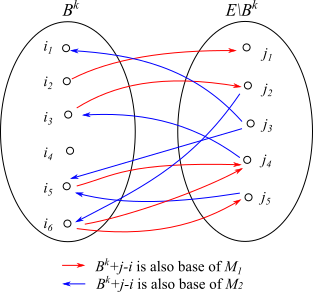
\includegraphics[width=6cm]{text8631-16-2-7.png}
 \end{figure}
\end{frame}

\begin{frame}{Finding all common bases in two matroids}
 \begin{figure}
  bipartite graph $G(B^k)$\\
  when $f = i_6$...\vspace{0.52cm}\\
  \centering
  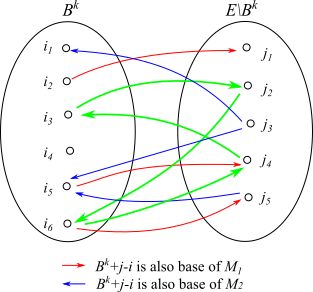
\includegraphics[width=6cm]{text8631-16-2-8.png}\\
 \end{figure}
\end{frame}

\begin{frame}{Finding all common bases in two matroids}
 \begin{figure}
  \centering
  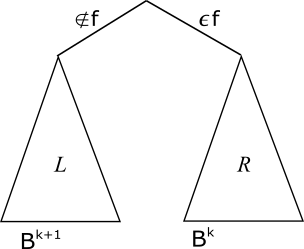
\includegraphics[width=4.5cm]{text8631-16-2-9.png}\\
  $\Updownarrow$ \\
  $B^k \cup \{j_3,\,j_4\}\setminus \{i_3,\,i_6\} \in \mathcal{B}_1 \cap \mathcal{B}_2$
 \end{figure}
\end{frame}

\begin{frame}{Finding all common bases in two matroids}
 simple algorithm example:\\
 $M_1 = M_2 = (E, \mathcal{B})$\\
 $E = \{1,\,2,\,3\}, \mathcal{B} = \{\{1,\,2\},\,\{2,\,3\}\}$\\
 $B^1 = \{2,\,3\}$
\end{frame}

\begin{frame}{Finding all common bases in two matroids}
 \begin{figure}
  \centering
  \hspace{0.2cm}
  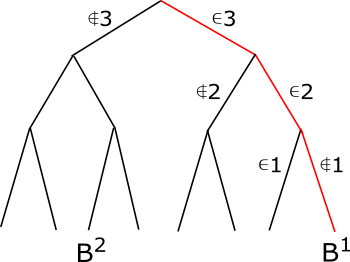
\includegraphics[width=5.2cm]{text4989.png}
 \end{figure}
 \begin{align*}
  &B^1 = \{2,\,3\}\\
  &P = (R\,R\,R)\\
  &P_1 = R \text{ then } f = 1
 \end{align*}
\end{frame}

\begin{frame}{Finding all common bases in two matroids}
 \begin{figure}
  \centering
  \hspace{0.1cm}
  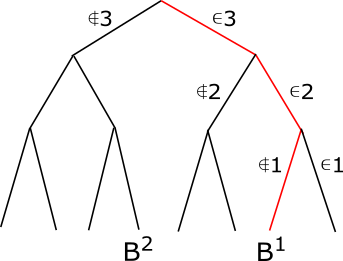
\includegraphics[width=5.1cm]{text4989-2.png}
 \end{figure}
 \begin{align*}
  &B^1 = \{2,\,3\}\\
  &P = (L\,R\,R)\\
  &P_2 = R \text{ then } f = 2
 \end{align*}
\end{frame}

\begin{frame}{Finding all common bases in two matroids}
 \begin{figure}
  \centering
  \hspace{0.03cm}
  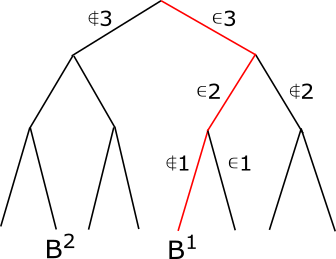
\includegraphics[width=5cm]{text4989-3.png}
 \end{figure}
 \begin{align*}
  &B^1 = \{2,\,3\}\\
  &P = (L\,L\,R)\\
  &P_3 = R \text{ then } f = 3
 \end{align*}
\end{frame}

\begin{frame}
 \begin{figure}
  \centering
  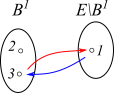
\includegraphics[width=2cm]{path16961.png}\\
  there exists an directed cycle $C$ in bipartite graph $G(B^1)$\\
  $\rightarrow$make pivot operation along $C$ and get new base $B^2 = \{1,\,2\}$ 
 \end{figure}
\end{frame}

\begin{frame}{Finding all common bases in two matroids}
 \begin{figure}
  \centering
  \hspace{0.03cm}
  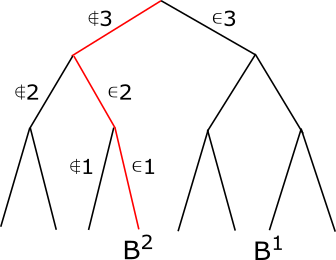
\includegraphics[width=5cm]{text4989-4.png}
 \end{figure}
 \begin{align*}
  &B^2 = \{1,\,2\}\\
  &P = (R\,R\,L)\\
  &P_1 = R \text{ then } f = 1
 \end{align*}
\end{frame}

\begin{frame}{Finding all common bases in two matroids}
 \begin{figure}
  \centering
  \hspace{0.2cm}
  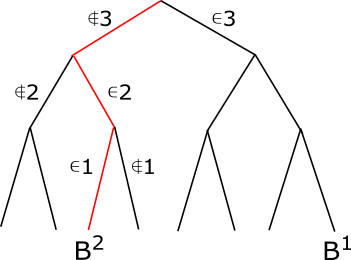
\includegraphics[width=5.2cm]{text4989-5.png}
 \end{figure}
 \begin{align*}
  &B^2 = \{1,\,2\}\\
  &P = (L\,R\,L)\\
  &P_2 = R \text{ then } f = 2
 \end{align*}
\end{frame}

\begin{frame}{Finding all common bases in two matroids}
 \begin{figure}
  \centering
  \hspace{-0.2cm}
  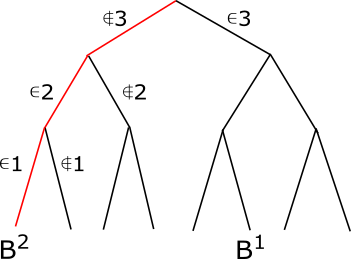
\includegraphics[width=5.2cm]{text4989-6.png}
 \end{figure}
 \begin{align*}
  &B^2 = \{1,\,2\}\\
  &P = (L\,L\,L)\\
  &f \text{ doesn't exist}\\
  &\text{end}
  \hspace{-0.1cm}
 \end{align*}
\end{frame}

\begin{frame}{Finding all common bases in two matroids}
 \begin{block}{alogrithm ``Enumerate''}
  input: $M_1 := (E,\,\mathcal{B}_1)$, $M_2 := (E,\,\mathcal{B}_2)$, $B^1 \in \mathcal{B}_1 \cap \mathcal{B}_2$\\
  output: all common bases of $M_1$ and $M_2$\\
  \begin{enumerate}
   \item $k := 1$, output $B^k$. $P := (R, ..., R)$. (Here, $P \in \{L,\,R\}^n$)
   \item $f := min\{j\,|\,\,P_j = R\}$
   \item If $f$ doesn't exist, stop. Else, create $G(B^k)$ and find directed cycle $C$ satisfying theorem 1 with breadth first search.
   \item If $C$ doesn't exist, goto step 2. Else, $k := k + 1$, make pivot operation along $C$ and obtain new $B^k$. $P_f := L$, $\forall j < k;\,P_j := R$, goto step 2.
  \end{enumerate}
 \end{block}
\end{frame}

\begin{frame}{Finding all common bases in two matroids}
 Again, $n = |E|$, $\lambda = |\mathcal{B}_1 \cap \mathcal{B}_2|$, and $t$ is time to generate $G(B^k)$.
 \begin{block}{time complexity}
  We evaluate the time from obtaining $B^k$ to obtaining $B^{k+1}$. Let $A_{max}$ be the maximum number of the arc in $G(B^k)$. Then $C$ in $G(B^k)$ satisfying Theorem 1 can be found in $O(A_{max})$ using BFS. This is iterated at most $n$ times(until finding such $C$). If such $C$ exists, then we pivot elements in $B^k$ along $C$ to get $B^{k+1}$ and generate $G(B^{k+1})$. This takes $O(C_{max}t)$ where $C_{max}$ is the length of the $C$.\\
  Since we know $A_{max} \leq (\frac{n}{2})^2 \cdot 2 = \frac{n^2}{2}$ and $C_{max}\leq 2 \cdot \frac{n}{2} = n$, it takes $O(n^3 + nt)$ from $B^k$ to $B^{k+1}$.\\
This is iterated $\lambda$ times, so total time complexity is $O((n^3 + nt)\lambda)$.
 \end{block}
  (note: $t$ depends on the imput form of the matroid. for example, the matroid is given in a form of a map, $t = O(n^2)$, but matroid is given in a form of a matrix, it's more than $n^2$)
\end{frame}

\section{Next step}
\begin{frame}{next month}
 TODO:
 \begin{enumerate}
  \item learn about matroid intersecrion
  \item learn how to partition a matoid into bases
  \item tackle two different partition matroids (can be partitioned into their common bases)
  \item generalized partition matroid of two different uniform matroids and any matroid
 \end{enumerate}
\end{frame}

\end{document}